\documentclass[11pt,letterpaper]{article}
\usepackage{graphicx, geometry, amsmath, hyperref, url, natbib, booktabs, xcolor, listings}
\usepackage{enumitem}
\geometry{margin=1in}
\hypersetup{colorlinks=true, linkcolor=black, citecolor=black, urlcolor=black}

\title{Executive Summary:\\Early Ego-Network Openness and Cross-Field Breadth of Scientific Concepts}
\author{AI Inventor}
\date{September 2026}

\begin{document}
\maketitle
\thispagestyle{empty}

\section*{Headline}

Scientific concepts whose early topic co-occurrence networks are more open---more diverse partners, more partner turnover, lower clustering---go on to spread across more disciplines. The OPEN\textsubscript{home} index, a composite of six ego-network indicators measured from home-field papers only, shows a partial Spearman correlation of $+0.069$ [$+0.038$, $+0.100$] with rarefied cross-field breadth, pooled over six non-selection bodies (four held-out field groups, a 2010--2014 onset cohort, and a fresh 2015--2017 onset cohort), with $I^2 = 0$ and 6/6 bodies positive. The association is modest (no practical forecasting gain over simple popularity features) but robust across fields and concept populations.

\section*{Goal}

Determine whether early structural signals in a scientific concept's topic co-occurrence network anticipate later cross-field breadth, beyond simple measures of volume and reach. The study uses the OpenAlex corpus (476 million works), tracking 12,499 concepts and 27,393 adoption episodes across 26 fields over a five-iteration research run.

\section*{What was tried}

\begin{enumerate}[nosep]
    \item \textbf{Iteration 1} screened five rival mechanisms (lineage naturalisation, co-author reach, co-occurrence diversity, frequency-free selectivity, gateway landing) on a 48-concept dev panel. None survived the pre-registered rule.
    \item \textbf{Iteration 2} scaled up to a 12,499-concept panel. Gateway centrality for retention was disconfirmed ($\Delta$AUC $= -0.00001$). Retained-field relatedness predicts field entry ($d_0 = 0.302$).
    \item \textbf{Iteration 3} ran the held-out indicator screen: 53 indicators, 10 frozen on DEV, 7 confirmed on held-out groups spanning two families (retained frontier and ego-network topology). Also ran the decisive retained-frontier test ($d_0 = 0.322$ on independent frame).
    \item \textbf{Iteration 4} confirmed OPEN on a fresh 2015--2017 cohort (marginal: $+0.080$ at R3, Holm $p = 0.048$). Breadth decomposition: 73\% exploration, 27\% retention. Within-concept closure test: NOT SUPPORTED.
    \item \textbf{Iteration 5} confirmed the signal on vocabulary-free ``Frame N'' concepts ($+0.117$ at R3); showed that Cheng's consistency predicts volume but \emph{narrower} reach ($-0.069$); found the signal is topical non-redundancy (static partner diversity), not year-to-year churn.
\end{enumerate}

\section*{Key results}

\begin{itemize}[nosep]
    \item Seven of 53 early network indicators survive held-out validation for rarefied breadth. They span two families: retained frontier (M0\_density\_end, D\_vol\_end, CONTACT\_REACH, RETENTION\_RATIO) and ego-network (n\_comm, NOV\textsubscript{res}, ego\_density).
    \item OPEN\textsubscript{home} PSP $+0.069$ [$+0.038$, $+0.100$] over 6 non-selection bodies ($I^2 = 0$).
    \item Retained-field relatedness predicts field entry: $d_0 = 0.322$ [$0.291$, $0.355$] on 6,978 entry events (FRONTIER = PARTIAL; backbone-specific).
    \item The consistency--breadth reversal: ideational consistency predicts volume ($+53.5\%$/SD) but narrower reach ($-0.069$; all five field groups negative, $I^2 = 0$).
    \item Breadth decomposition: early contact diversity accounts for 73\% of the gap; retention 27\%; frontier advance near zero.
    \item The signal is topical non-redundancy of the home-topic partner mix, not year-to-year partner turnover (within-concept permutation excess $+0.008 \approx 0$).
\end{itemize}

\begin{figure}[!htbp]
  \centering
  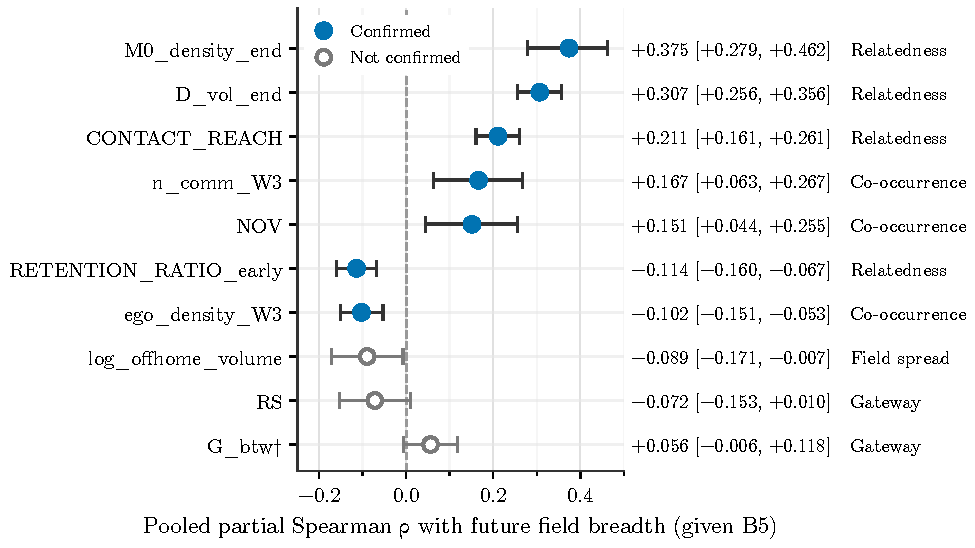
\includegraphics[width=\linewidth,height=0.85\textheight,keepaspectratio]{figures/fig_rq1_confirmed_v0.pdf}
  \caption{Held-out screen of the 10 indicators frozen on DEV for rarefied breadth. Seven are confirmed (filled circles, Holm $p < 0.05$): five positive, two negative.}
  \label{fig:rq1_exec}
\end{figure}

\section*{What failed}

\begin{itemize}[nosep]
    \item $A^*_h$ naturalisation gap, $D_\text{ratio}$, gateway landing $G$: fail on dev screen (iteration 1).
    \item Gateway centrality for retention: $\Delta$AUC $= -0.00001$ on 27,393 episodes (iteration 2).
    \item Trajectory typology: no discrete types pass the naming rule (ARI $= 0.222$).
    \item Within-concept closure (Experiment 11): NOT SUPPORTED; opposite sign on held-out.
    \item OPEN\textsubscript{home} forecasting gain: $+0.002$ over baseline---no practical prediction.
    \item Four artifacts failed or were incomplete across the run.
\end{itemize}

\section*{Open questions}

\begin{itemize}[nosep]
    \item The persistence-filtered RCA rival ($D_\text{rca\_persist\_k}$) remains untested.
    \item LIFEENV weakness (PSP $+0.071$ vs $+0.186$ for other bodies): unexplained.
    \item Causal mechanism: the association is correlational---openness could reflect intrinsic generality, community diversity, or problem breadth.
    \item Domain heterogeneity in field entry ($I^2 = 0.92$).
    \item Degree-normalised ego density and Palla size $\times$ turnover interaction were recommended but not run.
\end{itemize}

\end{document}
